{\bf Hardness}. We first show that Problem \ref{pr:revMax} (\RM) is NP-hard. We recall that a set function $f:2^U\ra \posreals$ is monotone if for $S\subset T\subseteq U$, $f(S) \le f(T)$. We define the marginal gain of an element $x$ w.r.t. $S\subset U$ as $f(x|S) := f(S\cup\{x\}) - f(S)$. A set function $f$ is submodular if for $S\subset T\subset U$ and $x\in U\setminus T$, $f(x|T) \le f(x|S)$, i.e., the marginal gains diminish with larger sets.

It is well known that the influence spread function $\sigma_i(\cdot)$ is monotone and submodular \cite{kempe03}, from which it follows that the  ad-specific revenue function $\pi_i(\cdot)$ is monotone and submodular. Finally, since the total revenue function, $\pi(\vecall) = \sum_{i \in [h]} \pi_i(S_i)$, is a non-negative linear combination of monotone and submodular functions, these properties carry over to $\pi(\vecall)$. Likewise, for each ad $i$, the payment function $\rho_i(\cdot)$ is a non-negative linear combination of two monotone and submodular functions, $\pi_i(\cdot)$ and $c_i(\cdot)$, and so is also monotone and submodular. Thus, the constraints $\rho_i(S_i) \le B_i$, $i\in[h]$, in Problem~\ref{pr:revMax} are submodular knapsack constraints. We start with our hardness result.
%For lack of space, we omit all proofs except that of the major result, Theorem~\ref{theo:cs-earm1}. The complete details of all proofs can be found in \cite{us-arxiv}.

\begin{theorem}\label{claim:npHard}
Problem \ref{pr:revMax} (\RM) is \NPhard.
\end{theorem}

\begin{proof}
Consider the special case with one advertiser, i.e., $h = 1$. Then we have one submodular knapsack constraint and no partition matroid constraint. This corresponds to maximizing a submodular function subject to a submodular knapsack constraint, the so-called Submodular Cost Submodular Knapsack (SCSK) problem, which is known to be NP-hard~\cite{iyer2013submodular}. Since this is a special case of Problem \ref{pr:revMax}, the claim follows.
\end{proof}

Next, we characterize the constraint that the allocation $\vecall = (S_1, \cdots, S_h)$ should be composed of pairwise disjoint sets, i.e., $S_i \cap S_j = \emptyset , i \neq j, \forall i,j \in [h]$. We will make use of the following notions on matroids.
\enlargethispage{2\baselineskip}

\begin{definition}[Independence System]\label{def:IS}
A set system $(\mathcal{E},\mathcal{I})$ defined with a finite ground set $\mathcal{E}$ of elements, and a family $\mathcal{I}$ of subsets of $\mathcal{E}$ is an independence system if $\calI$ is non-empty and if it satisfies downward closure axiom, i.e.,
$X \in \mathcal{I} \wedge Y \subseteq X \rightarrow Y \in \mathcal{I}$.


%\squishlist
% \item %$\emptyset \in \mathcal{I}$.
%$\calI$ is non-empty.
% \item {\bf Downward Closure}: If $X \in \mathcal{I}$ and $Y \subseteq X$, then $Y \in \mathcal{I}$.
%\squishend
\end{definition}

\begin{definition}[Matroid]\label{def:Matroid}
An independence system $(\mathcal{E}, \mathcal{I})$ is a matroid $\mathfrak{M} = (\mathcal{E}, \mathcal{I})$ if it also satisfies the augmentation axiom: i.e.,
$X \in \mathcal{I} \wedge Y \in \mathcal{I} \wedge |Y| > |X| \rightarrow \exists e \in Y \setminus X : X \cup \{e\} \in \mathcal{I}$.
%\squishlist
% \item {\bf Augmentation}: If $X \in \mathcal{I}$ and $Y \in \mathcal{I}$ and $|Y| > |X|$, then $\exists e \in Y \setminus X : X \cup \{e\} \in \mathcal{I}$.
%\squishend
\end{definition}

\begin{definition}[Partition Matroid]\label{def:PartitionMatroid}
Let $\mathcal{E}_1, \cdots, \mathcal{E}_l$ be a partition of the ground set $\mathcal{E}$ into $l$ non-empty disjoint subsets. Let $d_i$ be an integer, $0 \le d_i \le |\mathcal{E}_i|$. In a partition matroid $\mathfrak{M} = (\mathcal{E}, \mathcal{I})$, a set $X$ is defined to be independent iff, for every $i$, $1\le i\le l$, $|X \cap \mathcal{E}_i| \le d_i$. That is, $\mathcal{I} = \{X \subseteq \mathcal{E} : |X \cap \mathcal{E}_i| \le d_i, \forall i = 1,\cdots,l \}$.
\end{definition}

%%%\begin{definition}[Ranks]\label{def:ISRankDefs}
%%%Let $(\mathcal{E}, \mathcal{I})$ be an independence system and $X \subseteq \mathcal{E}$ be an arbitrary subset. The lower and upper rank of $X$ in $(\mathcal{E}, \mathcal{I})$  are the cardinalities of the smallest and largest maximal independent sets in $X$.
%%%$$r(X) =  \text{min}\{|Y| : Y \subseteq X, Y \in \mathcal{I} \text{ and }  Y \cup \{e\} \not\in \mathcal{I}, \forall x \in X \setminus Y \},$$
%%%$$R(X) =  \text{max}\{|Y| : Y \subseteq X, Y \in \mathcal{I} \}.$$
%%%%\squishlist
%%%%\item$r(X) =  \text{min}\{|Y| : Y \subseteq X, Y \in \mathcal{I} \text{ and }  Y \cup \{e\} \not\in \mathcal{I}, \forall x \in X \setminus Y \},$
%%%%\item $R(X) =  \text{max}\{|Y| : Y \subseteq X, Y \in \mathcal{I} \text{ and }  Y \cup \{e\} \not\in \mathcal{I}, \forall x \in X \setminus Y \}.$
%%%%\squishend
%%%The lower and upper rank of the independence system $(\mathcal{E}, \mathcal{I})$ are respectively defined by $r = r(\mathcal{E})$ and $R = R(\mathcal{E})$.
%%%\end{definition}
%%%
%%%\begin{definition}[Rank quotient]\label{def:ISRQuot}
%%%The rank quotient $q(\mathcal{E}, \mathcal{I})$ of an independence system $(\mathcal{E}, \mathcal{I})$ is given by:
%%%$$ q(\mathcal{E}, \mathcal{I}) = \underset{S \subseteq \mathcal{E}}{\text{min }}{\dfrac{r(S)}{R(S)}}.$$
%%%$q(\mathcal{E}, \mathcal{I})$ measures how much $(\mathcal{E}, \mathcal{I})$ differs from being a matroid: $(\mathcal{E}, \mathcal{I})$ is a matroid iff $q(\mathcal{E}, \mathcal{I}) = 1$.
%%%\end{definition}

%We next show that the constraint that in an allocation, the seed sets $S_i$ must be pairwise disjoint, corresponds to a partition matroid constraint.

\begin{lemma}\label{lem:matroid}
The constraint that in an allocation $\vecall = (S_1, \cdots, S_h)$, the seed sets $S_i$ are pairwise disjoint is a partition matroid constraint over the ground set $\mathcal{E}$ of all (node, advertiser) pairs.
\end{lemma}

%%%%%%%%%%%%%%%%%%%%%%%%% include in arxiv start
%\eat{
\begin{proof}
Given $G=(V,E)$, $\Card{V} = n$, and a set $A = \{i : i \in [h] \}$ of advertisers, let $\mathcal{E} = V \times A$ denote the ground set of all $(node, advertiser)$ pairs. Define $\mathcal{E}_u = \{ (u,i) : i \in A \}$, $u \in V$. Then the set $\{\mathcal{E}_u : \forall u \in  V \}$ forms a partition of $\mathcal{E}$ into $n$ disjoint sets, i.e., $\mathcal{E}_u \cap \mathcal{E}_v = \emptyset$, $u \ne v$, and $\bigcup_{u \in V} \mathcal{E}_u = \mathcal{E}$. Given a subset $\mathcal{X} \subseteq \mathcal{E}$, define
\begin{align*}
S_i = \{u : (u,i) \in \mathcal{X}\}.
\end{align*}
Then it is easy to see that the sets $S_i, i\in [h]$ are pairwise disjoint iff the set $\mathcal{X}$ satisfies the constraint
\begin{align*}
\mathcal{X} \cap \mathcal{E}_u \le 1, \forall u\in V.
\end{align*}

The lemma follows on noting that the set system $\mathfrak{M} = (\mathcal{E}, \mathcal{I})$, where $\mathcal{I} = \{\mathcal{X} \subseteq \mathcal{E} : |\mathcal{X}\cap\mathcal{E}_u| \le 1, \forall u \in V\}$ is actually a partition matroid.
\end{proof}
%}
%%%%%%%%%%%%%%%%%%%%%%%%% include in arxiv end

 Therefore, the \RM problem corresponds to the problem of submodular function maximization subject to a partition matroid constraint $\mathfrak{M} = (\mathcal{E}, \mathcal{I})$, \emph{and} $h$ submodular knapsack constraints.

\spara{Approximation analysis.}
Next lemma states that the constraints of the \RM problem together form an independence system defined on the ground set $\mathcal{E}$. This property will be leveraged later in developing approximation algorithms.
% of $(node, advertiser)$ pairs.
Given the partition matroid constraint $\mathfrak{M} = (\mathcal{E}, \mathcal{I})$, and $h$ submodular knapsack constraints, let $\mathcal{C}$ denote the family of subsets, defined on $\mathcal{E}$, that are feasible solutions to the \RM problem.

\begin{lemma}\label{lem:IS}
The system $(\calE, \calC)$ is an independence system.
\end{lemma}

%%%%%%%%%%%%%%%%%%%%%%%%% include in arxiv start
%\eat{
\begin{proof}
 For each knapsack constraint $\rho_i(\cdot) \le B_i$, let $\mathcal{F}_i \subseteq 2^V$ denote the collection of feasible subsets of $V$, i.e.,
\begin{align*}
\mathcal{F}_i = \{ S_i \subseteq V : \rho_i(S_i) \le B_i \}.
\end{align*}
The set system $(V,\mathcal{F}_i)$ defined by the set of feasible solutions to any knapsack constraint is downward-closed, hence is an independence system. Given $\mathcal{F}_i$, $\forall i \in [h]$ and the partition matroid constraint $\mathfrak{M} = (\mathcal{E}, \mathcal{I})$, we can define the family of subsets of $\mathcal{E}$ that are feasible solutions to the \RM problem as follows:
\begin{align*}
\mathcal{C} = \left\{ \mathcal{X} : \mathcal{X} \in \mathcal{I} \text{ and } S_i \in \mathcal{F}_i, \forall i \in [h]  \right\}
\end{align*}
where $S_i = \{ u : (u,i) \in \mathcal{X} \}$. Let $\mathcal{X} \in \mathcal{C}$ and $\mathcal{X}' \subseteq \mathcal{X}$. In order to show that $\mathcal{C}$ is an independence system, it suffices to show that $\calX'\in \calC$.

Let $S_i' = \{ u : (u, i) \in \mathcal{X}' \} $, $i  \in [h]$.
Clearly, $S_i' \subseteq S_i$. As each single knapsack constraint $\rho_i(\cdot) \le B_i$ is associated with the independence system $(V, \mathcal{F}_i)$, we have $S_i' \in \mathcal{F}_i$ for any $S_i' \subseteq S_i$, $i \in [h]$.

Next, as $\mathcal{X} \in \mathcal{I}$, we have $S_i \cap S_j = \emptyset$.
Since $\mathfrak{M} = (\calE, \calI)$ is a partition matroid, by downward closure, $\calX' \in \calI$, and hence $S_i'\cap S_j' = \emptyset$, $i \ne j$.
\eat{
Given the one-to-one correspondence between $S_i'$ and $\mathcal{X}'$, and $\mathcal{X}' \in \mathcal{I}$ due to the downward closure property of the partition matroid $\mathfrak{M}$.
}
We just proved $\calX' \in \calC$, verifying that $\calC$ is an independence system.

\end{proof}
%}
%%%%%%%%%%%%%%%%%%%%%%%%% include in arxiv end
Our theoretical guarantees for our approximation algorithms to the \RM problem depend on the notion of \emph{curvature} of submodular functions. Recall that $f(j|S)$, $j\not\in S$, denotes the marginal gain $f(S\cup\{j\}) - f(S)$.
\begin{definition}[Curvature]\cite{conforti1984submodular}
Given a submodular function $f$, the total curvature $\kappa_f$ of $f$ is defined as
\begin{align*}
\kappa_f = 1 - \underset{j \in V} {\min} \dfrac{f(j|V\setminus\{j\})}{f(\{j\})},
\end{align*}
and the curvature $\kappa_f(S)$ of $f$ wrt a set $S$ is defined as
\begin{align*}
\kappa_f(S) = 1 - \underset{j \in S} {\min} \dfrac{f(j|S\setminus\{j\})}{f(\{j\})}.
\end{align*}
\end{definition}
It is easy to see that $0 \le \kappa_f = \kappa_f(V) \le 1$. Intuitively, the curvature of a function measures the deviation of $f$ from \emph{modularity}: modular functions have a curvature of $0$, and the further away $f$ is from modularity, the larger $\kappa_f$ is. Similarly, the curvature $\kappa_f(S)$ of $f$ \emph{wrt} a set $S$ reflects how much the marginal gains $f(j \mid S)$ can decrease as a function of $S$, measuring the deviation from modularity, given the context $S$.
%%%%%%%%%%%%%%%%%%%%%%%%% include in arxiv start
%\eat{
Iyer et al.~\cite{iyer2015submodularthesis} introduced the notion of \emph{average} curvature $\hat{\kappa}_f(S)$ of $f$ wrt a set $S$ as
\begin{align*}
\hat{\kappa}_f(S) = 1 - \dfrac{\sum_{j \in S} f(j|S \setminus\{j\} )}{\sum_{j \in S} f(\{j\})},
\end{align*}
and showed the following relation between these several forms of curvature:
\begin{align*}
 0 \le \hat{\kappa}_f(S) \le \kappa_f(S)  \le \kappa_f(V) = \kappa_f \le 1.
\end{align*}
%}
%%%%%%%%%%%%%%%%%%%%%%%%% include in arxiv end
In the next subsections, we propose two greedy approximation algorithms for the \RM problem. The first of these, Cost-Agnostic Greedy Algorithm (\CARM), greedily chooses the seed users solely based on the marginal gain in the revenue, without considering seed user incentive costs. The second, Cost-Sensitive Greedy Algorithm (\CSRM), greedily chooses the seed users based on the \emph{rate} of marginal gain in revenue per marginal gain in the advertiser's payment for each advertiser.

We note that Iyer et al. \cite{iyer2013submodular, iyer2015submodularthesis} study a restricted special case of the \RM problem, referred as Submodular-Cost Submodular-Knapsack (SCSK), and propose similar cost-agnostic and cost-sensitive algorithms. Our results extend theirs in two major ways. First, we extend from a single advertiser to multiple advertisers (i.e., from
a single submodular knapsack constraint to multiple submodular knapsack constraints). Second, unlike SCSK, our \RM problem is  subject to an additional partition matroid constraint on the ads-to-seeds allocation, which naturally arises when multiple advertisers are present.

\enlargethispage{2\baselineskip}
\subsection{Cost-Agnostic Greedy Algorithm}
The Cost-Agnostic Greedy Algorithm (\CARM) for the \RM problem, whose pseudocode is provided in Algorithm~\ref{alg:CA-EARM}, chooses at each iteration a (node, advertiser) pair that provides the maximum increase in the revenue of the host.
Let $\mathcal{X}_g \subseteq \mathcal{E}$ denote the greedy solution set of (node,advertiser) pairs, returned by \CARM,  having one-to-one correspondence with the greedy allocation $\vecalloc$, i.e., $S_i = \{u : (u,i) \in \mathcal{X}_g \}$, $\forall S_i \in \vecalloc$. Let $\mathcal{X}_g^t$ denote the greedy solution after $t$ iterations of \CARM. At each iteration $t$, \CARM first finds the (node,advertiser) pair $(u^*,i^*)$ that maximizes  $\pi_i(u \mid S^{t-1}_i)$, and tests whether adding this pair to the current greedy solution $\mathcal{X}_g^{t-1}$ would violate any constraint: if $\mathcal{X}_g^{t-1} \cup \{(u^*,i^*)\}$ is feasible, the pair $(u^*,i^*)$ is added to the greedy solution as the $t$-th (node,advertiser) pair. Otherwise, $(u^*,i^*)$ is removed from the current ground set of (node,advertiser) pairs $\mathcal{E}^{t-1}$. \CARM terminates when there is no feasible (node,advertiser) pair left in the current ground set $\mathcal{E}^{t-1}$.

\begin{observation}\label{obs:curvatureTotalPi}
Being monotone and submodular, the total revenue function $\pi(\vecalloc)$ has a total curvature $\kappa_{\pi}$, given by: %on the ground set $\mathcal{E}$:
\begin{align*}
\kappa_{\pi} = 1 - \underset{(u,i) \in \mathcal{E}} {\min} \dfrac{\pi_i(u \mid V \setminus\{u\})}{\pi_i(\{u\})}.
\end{align*}
\end{observation}

%%%%%%%%%%%%%%%%%%%%%%%%% include in arxiv start
%\eat{
\begin{proof}
Let $g : 2^{\mathcal{E}} \mapsto \mathbb{R}_{\ge 0}$ be monotone and submodular. % defined on the ground set $\mathcal{E}$.
Then, the total curvature $\kappa_g$ of $g$ is defined as follows:
\begin{align*}
\kappa_g = 1 - \underset{x \in \mathcal{E}} {\min} \dfrac{g(x \mid \mathcal{E} \setminus\{x\} )}{g(\{x\})},
\end{align*}
where $x = (u,i) \in \mathcal{E}$. Using the one-to-one correspondence between $\mathcal{X}_g$ and $\vecalloc$, we can alternatively formulate the \RM problem as follows:

\begin{equation*}
\begin{aligned}
& \underset{\mathcal{X} \subseteq \mathcal{E}}{\text{maximize}}
& & g(\mathcal{X}) \\
& \text{subject to}
& & \mathcal{X} \in \mathcal{C}.  \\
\end{aligned}
\end{equation*}
where $g(\mathcal{X}) = \sum_{i \in [h]} \pi_i(S_i)$ with $S_i = \{ u : (u,i) \in \mathcal{X} \}$. \\

Using this correspondence, we can rewrite $\kappa_g$ as $\kappa_{\pi}$ as follows:
\begin{align*}
\kappa_g = \kappa_{\pi} = 1 - \underset{(u,i) \in \mathcal{E}} {\min} \dfrac{\pi_i(\{u\} \mid V \setminus\{u\})}{\pi_i(\{u\})}.
\end{align*}
\end{proof}
%}
%%%%%%%%%%%%%%%%%%%%%%%%% include in arxiv end
We will make use of the following notions in our results on approximation guarantees.
%
\begin{definition}[Upper and lower rank]
Let $({\cal E}, {\cal C})$ be an independence system. Its \emph{upper rank} $R$ and \emph{lower rank} $r$ are defined as the cardinalities of the smallest and largest maximal independent sets:
$$r = \min \{|X| : X \in \mathcal{C} \text{ and } X \cup \{(u,i)\} \not\in \mathcal{C}, ~\forall (u,i) \not\in X\}, $$
$$R = \max \{|X| : X \in \mathcal{C} \text{ and } X \cup \{(u,i)\} \not\in \mathcal{C}, ~\forall (u,i) \not\in X\}.$$
\end{definition}

When the independence system is a matroid, $r=R$, as all maximal independent sets have the same cardinality.
\begin{theorem}\label{theo:CARM}
\CARM achieves an approximation guarantee of $\dfrac{1}{\kappa_{\pi}}\left[ 1- \left(\dfrac{R - \kappa_{\pi}}{R}\right)^{r} \right]$ to the optimum, where $\kappa_{\pi}$ is the total curvature of the total revenue function $\pi(\cdot)$, $r$ and $R$ are respectively the lower and upper rank of $(\mathcal{E}, \mathcal{C})$. \LL{This bound is tight}.
\eat{
, \emph{i.e.}, the cardinalities of the smallest and largest maximal independent sets in $\mathcal{C}$:
$$r = \min \{|X| : X \in \mathcal{C} \text{ and } X \cup \{(u,i)\} \not\in \mathcal{C}, ~\forall (u,i) \not\in X\}, $$
$$R = \max \{|X| : X \in \mathcal{C} \text{ and } X \cup \{(u,i)\} \not\in \mathcal{C}, ~\forall (u,i) \not\in X\}.$$
}
\end{theorem}


\begin{proof}
We note that the family $\mathcal{C}$ of subsets that constitute \emph{feasible} solutions to the \RM problem form an independence system defined on $\mathcal{E}$ (Lemma~\ref{lem:IS}). Given this, the approximation guarantee of \CARM directly follows from the result of Conforti et al.~\cite[Theorem 5.4]{conforti1984submodular} for submodular function maximization subject to an independence system constraint. \LL{However, the tightness does \emph{not} directly follow from the tightness result in \cite{conforti1984submodular}, which we address next.}

\LL{We now exhibit an instance to show that the bound is tight. Consider one advertiser, i.e., $h = 1$. The network is shown in Figure~\ref{fig:tightness}, where all influence probabilities are $1$. The incentive costs for nodes are as shown in the figure, while $cpe(.) = 1$. The budget is $B=7$.  It is easy to see that the lower rank is $r = 1$, corresponding to the maximal feasible seed set $S = \{b\}$, while the upper rank is $R = 2$, e.g., corresponding to  maximal feasible seed sets such as $T = \{a, c\}$. Furthermore, the total curvature is $\kappa_{\pi} = 1$. On this instance, the optimal solution is $T$ which achieves a revenue of $6$. In its first iteration, \CARM could choose $b$ as a seed. Once it does, it is forced to the solution $S = \{b\}$ as no more seeds can be added to $S$. The revenue of \CARM is $3 = \dfrac{1}{\kappa_{\pi}}\left[ 1- \left(\dfrac{R - \kappa_{\pi}}{R}\right)^{r} \right]OPT = \frac{1}{2} \cdot 6$. }
 \end{proof}

%%%%%%%%%%%%%%%%%%%%%%%%%%%%
\begin{figure}[t!]
\vspace{-4mm}
\centering{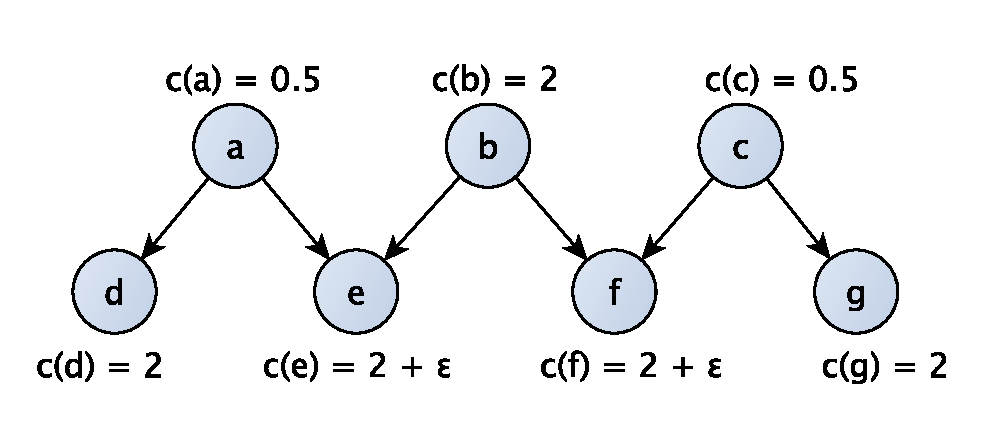
\includegraphics[width=.39\textwidth, height=.12\textheight]{toy_tightness_ntw.pdf}}
\vspace{-4mm}
\caption{Instance illustrating tightness of bound in Theorem~\ref{theo:CARM}.}
\label{fig:tightness}
\vspace{2mm}
\end{figure}
%%%%%%%%%%%%%%%%%%%%%%%%%%%%

\noindent \LL{\textbf{Discussion.} We next discuss the significance and the meaning of the bound in Theorem~\ref{theo:CARM}. 
Notice that when there is just one advertiser, TIC reduces to IC. Even for this simple setting, the bound on \CARM is tight.
By a simple rearrangement of the terms, we have:
$$\dfrac{1}{\kappa_{\pi}}\left[ 1- \left(\dfrac{R - \kappa_{\pi}}{R}\right)^{r} \right] \ge \dfrac{1}{\kappa_{\pi}} \left( 1 - e^{ - \kappa_{\pi} \cdot \dfrac{r}{R}} \right).
$$
%\begin{align*}
% \dfrac{1}{\kappa_{\pi}}\left[ 1- \left(\dfrac{R - \kappa_{\pi}}{R}\right)^{r} \right] &= \dfrac{1}{\kappa_{\pi}}\left[ 1- \left(1 - \dfrac{ \kappa_{\pi}}{R}\right)^{r} \right] \\ &\ge \dfrac{1}{\kappa_{\pi}} \left( 1 - e^{ - \kappa_{\pi} \cdot \dfrac{r}{R}} \right).
%\end{align*}
%where the last inequality is obtained from the fact that $1- x \le e^{-x}$, hence, $\left(1 - \dfrac{\kappa_{\pi}}{R} \right)^r \le \left(e^{-\dfrac{\kappa_{\pi}}{R}}\right)^r$.
Clearly, the cost-agnostic approximation bound improves as $\dfrac{r}{R}$ approaches $1$, achieving the best possible value when $r = R$. As a special case, the cost-agnostic approximation further improves when the independence system $(\mathcal{E}, \mathcal{C})$ is a matroid since for a matroid $r = R$ always holds: e.g., consider the standard IM problem~\cite{kempe03} which corresponds to submodular function maximization subject to a uniform matroid. Here, $\pi(\cdot) = \sigma(\cdot)$.
Then the %cost-agnostic
approximation guarantee becomes $\dfrac{1}{\kappa_{\pi}} \left( 1 - e^{ - \kappa_{\pi}} \right)$, providing a slight improvement over the usual $(1 - 1/e)$-approximation, thanks to the curvature term $\kappa_{\pi}$.\footnote{\small \LL{Note that $\kappa_{\pi} \le 1$ always. Hence, the extent of improvement increases as the total curvature $\kappa_{\pi}$ decreases.}} This remark is also valid for budgeted influence maximization~\cite{LeskovecKDD07} with uniform seed costs. }
%
%\note[Laks]{Need to improve the message below.}
\LL{For more general instances of the problem, the guarantee depends on the characteristics of the instance, specifically, the lower and upper ranks and the curvature. This kind of instance dependent bound is characteristic of submodular function maximization over an independence system~\cite{korte78,conforti1984submodular}. Specifically for the RM problem, given its constraints, the values of $r$ and $R$ are dictated by the values of $h$ payment functions over all feasible allocations. For instance, given our assumption that every advertiser can afford at least one seed, we always have $r \ge h$. The worst-case value $r = h$ corresponds to the case in which each advertiser $i$ is allocated a single seed node $u_i$ whose payment $\rho_i(u_i)$ exhausts its budget $B_i$. Similarly for $R$, without using any particular assumption on $B_i$, $\forall i \in [h]$, we always have $R \le \text{min}(n, \sum_{i \in [h]} \left\lfloor B_i / cpe(i) \right\rfloor)$.}
%%%%%%%%%%%%%%%%%%%%%%%%% include in arxiv start
%\eat{
\CA{Notice also that:
\begin{align}
\dfrac{1}{\kappa_{\pi}}\left[ 1- \left(\dfrac{R - \kappa_{\pi}}{R}\right)^{r} \right] &= \dfrac{1}{\kappa_{\pi}}\left[ 1- \left(1 - \dfrac{ \kappa_{\pi}}{R}\right)^{r} \right] \\
\ge  \dfrac{1}{\kappa_{\pi}} \left[ 1- \left(1 - \dfrac{ \kappa_{\pi}}{R}\right) \right] &= \dfrac{1}{\kappa_{\pi}} \dfrac{ \kappa_{\pi}}{R} = \dfrac{1}{R}
\end{align}
Hence, the worst-case approximation is always bounded by $1/R$.}
%}
%%%%%%%%%%%%%%%%%%%%%%%%% include in arxiv end

%\note[Laks]{Please see my pinned comments in the revision channel.}

\begin{algorithm}[!h!]
 \caption{\CARM}
%\label{alg:greedyEnvyAgnostic}
\label{alg:CA-EARM}
{\small
\SetKwInOut{Input}{Input}
\SetKwInOut{Output}{Output}
\SetKwComment{tcp}{//}{}
% \Input{$G=(V,E)$, $\mathcal{E}$, $\mathcal{C}$, $B_i$, $\cpe{i}$, $\vec{\gamma}_i, \forall i \in [h]$, $c_i(u), \forall u \in V$}
\Input{$G=(V,E)$, $B_i$, $\cpe{i}$, $\vec{\gamma}_i, \forall i \in [h]$, $c_i(u), \forall i \in [h], \forall u \in V$}
 \Output{$\vecalloc = (S_1, \cdots, S_h)$}
} % small \\
%Assume wlog that  $v_1 \succ v_2 \succ \cdots \succ v_h \succ r_{min}$ \\
{\small
$t \leftarrow 1$, $\mathcal{E}^0 \leftarrow \mathcal{E}$, $\mathcal{X}_g^0 \leftarrow \emptyset$ \\
$S^0_i \leftarrow \emptyset$, $\forall i \in [h]$ \\
}
\While{$\mathcal{E}^{t-1} \neq \emptyset$} {
$(u^*,i^*) \leftarrow \argmax_{(u,i) \in \mathcal{E}^{t-1}}  \pi_i(u \mid S^{t-1}_i)$ \\ \label{line:greedyCriteria}
\uIf{$(\mathcal{X}_g^{t-1} \cup \{(u^*,i^*)\}) \in \mathcal{C}$} {
%\uIf{$\rho(S_{i_t}^{t-1} \cup \{u_t \}, p_{i_t}) \le B_{i_t}$} {
			$S_{i^*}^{t} \leftarrow S_{i^*}^{t-1} \cup \{ u^*\} $ \\
			$S_j^t \leftarrow S_j^{t-1}$, $\forall j \neq i^*$ \\
			$\mathcal{X}_g^{t} \leftarrow \mathcal{X}_g^{t-1} \cup \{(u^*, i^*)\}$ \\
			$\mathcal{E}^t \leftarrow \mathcal{E}^{t-1} \setminus \{(u^*, i^*)\}$ \\
			$t \leftarrow t + 1$ \\
%}
}
\uElse{
$\mathcal{E}^{t-1} \leftarrow \mathcal{E}^{t-1} \setminus \{(u^*, i^*)\} $ \\
}
}
$S_i \leftarrow S^{t-1}_i$, $\forall i \in [h]$ \\
{\bf return} $\vecalloc = (S_1, \cdots, S_h)$
\end{algorithm}

\vspace{2mm} \subsection{Cost-Sensitive Greedy Algorithm}
The Cost-sensitive greedy algorithm (\CSRM) for the \RM problem is similar to \CARM. The main difference is that at each iteration $t$, \CSRM first finds the (node,advertiser) pair $(u^*,i^*)$ that maximizes $\dfrac{\pi_i(u \mid S^{t-1}_i)}{\rho_i(u \mid S^{t-1}_i)} $, and tests whether the addition of this pair to the current greedy solution set $\mathcal{X}_g^{t-1}$ would violate any matroid or knapsack independence constraint: if the addition is feasible, %\emph{i.e.}, $\mathcal{X}^{t-1}_g \cup \{(u^*,i^*)\} \in \mathcal{C}$,
the pair $(u^*,i^*)$ is added to the greedy solution as the $t$-th (node,advertiser) pair. Otherwise, $(u^*,i^*)$ is removed from the current ground set %of $(node,advertiser)$ pairs
$\mathcal{E}^{t-1}$.
%, as it violates either the partition matroid constraint or the knapsack constraint.
\CSRM terminates when there is no (node,advertiser) pair left in the current ground set $\mathcal{E}^{t-1}$. \CSRM can be obtained by simply replacing Line~\ref{line:greedyCriteria} of Algorithm~\ref{alg:CA-EARM} with
$$ (u^*,i^*) \leftarrow \underset{(u,i) \in \mathcal{E}^{t-1}} \argmax \dfrac{\pi_i(u \mid S^{t-1}_i)}{\rho_i(u \mid S^{t-1}_i)}. $$
%thus, we do not provide the pseudocode due to lack of space.

% the declaration of the initial guarantee we had before
%\begin{theorem}\label{theo:cs-earm1}
%\CSRM achieves an approximation guarantee of $$  \left(1 + \dfrac{B}{\Delta \rho_{min} \cdot (1 - \underset{i \in [h]} {\text{max }} \hat{\kappa}_{\rho_i}(S^*_i))} \right)^{-1} $$ where $\vec{S^*} = (S_1^*, \cdots, S_h^*)$ is the optimal allocation, $\vecalloc = (S_1, \cdots, S_h)$ is the greedy allocation, $B = \sum_{i \in [h]} B_i$ is the total input budget, $K = {\bigcup}_{i \in [h]} \Card{S_i}$ is the size of the greedy solution, $\Delta  \rho_{min} := {\min}_{i \in [h], t \in [1,K]} \rho_i(S_i^t) - \rho_i(S_i^{t-1})$, \emph{i.e.}, minimum marginal gain in payment obtained in an iteration of the greedy algorithm, and $\hat{\kappa}_{\rho_i}(S^*_i)$ is the average curvature of $\rho_i(\cdot)$ wrt $S_i^*$, $i \in [h]$.
%\end{theorem}

\begin{theorem}\label{theo:cs-earm1}
\CSRM achieves an approximation guarantee of
$$1 - \dfrac{R \cdot \rho_{max} }{R \cdot \rho_{max} + (1 - \underset{i \in [h]} {\text{max }} {\kappa_{\rho_{i}}}) \cdot \rho_{min}} $$
 to the optimum where $R$ is the upper rank of $(\mathcal{E}, \mathcal{C})$, $\kappa_{\rho_{i}}$ is the total curvature of $\rho_i(\cdot)$, $\forall i \in [h]$,  $\rho_{max} := \underset{(u,i) \in \mathcal{E}} {\text{max }} \rho_{i}(u) $ and $\rho_{min} := \underset{(u,i) \in \mathcal{E}} {\text{min }} \rho_{i}(u) $ are respectively the maximum and minimum singleton payments over all (node, advertiser) pairs.
\end{theorem}
\begin{proof}
We use $\vec{S^*} = (S_1^*, ..., S_h^*)$ and $\vecalloc = (S_1, ..., S_h)$ to denote the optimal and greedy allocations respectively, and $\calX^*$ and $\calX_g$ to denote the corresponding solution sets. Specifically, $S_i^* = \{u : (u,i) \in \mathcal{X}^*\}$, and $S_i = \{u : (u,i) \in \mathcal{X}_g \}$. We denote by $\calX_g^t$ the result of the greedy solution after $t$ iterations. Let $K = |\mathcal{X}_g|$ denote the size of the greedy solution. Thus, $\calX_g = \calX_g^K$. By submodularity and monotonicity:
\begin{small}
$$\pi(\vec{S^*}) \le \pi(\vecalloc)  + \sum_{(u,i) \in \mathcal{X}^* \setminus \mathcal{X}_g} \pi_i(u \mid S_i) \le \pi(\vecalloc)  + \sum_{(u,i) \in \mathcal{X}^*} \pi_i(u \mid S_i).$$
\end{small}
At each iteration $t$, the greedy algorithm first finds the (node, advertiser) pair $(u^*,i^*) \leftarrow \underset{(u,i) \in \mathcal{E}^{t-1}} \argmax \dfrac{\pi_i(u \mid S^{t-1}_i)}{\rho_i(u \mid S^{t-1}_i)}$, and tests whether the addition of this pair to the current greedy solution set $\mathcal{X}_g^{t-1}$ would violate any independence constraint. If $(u^*,i^*)$ is feasible, i.e., if $\mathcal{X}_g^{t-1} \cup \{(u^*,i^*)\} \in \mathcal{C}$, then the pair $(u^*,i^*)$ is added to the greedy solution as the $t$-th (node, advertiser) pair; otherwise, $(u^*,i^*)$ is removed from the current ground set $\mathcal{E}^{t-1}$. In what follows, for clarity, we use the notation $(u_t, i_t)$ to denote the (node, advertiser) pair that is \emph{successfully} added by the greedy algorithm to $\mathcal{X}_g^{t-1}$ in iteration $t$.

Let $U^{t}$ denote the set of (node, advertiser) pairs that the greedy algorithm \emph{tested} for possible addition to the greedy solution in the first $(t+1)$ iterations \emph{before} the addition of the $(t+1)$-st pair $(u_{t+1}, i_{t+1})$ into $\mathcal{X}_g^{t}$. Thus, $U^t \setminus U^{t-1}$ includes the $t$-th pair $(u_t, i_t)$ that was successfully added to $\mathcal{X}_g^{t-1}$, as well as all the pairs that were tested for addition into $\mathcal{X}_g^{t}$ but failed the independence test. Thus, $\forall (u,i) \in U^t \setminus U^{t-1}$, we have
$\dfrac{\pi_{i}(u \mid S_{i}^{t})}{\rho_{i}(u \mid S_{i}^{t})} \ge \dfrac{\pi_{i_{t+1}}(u_{t+1} \mid S_{i_{t+1}}^{t})}{\rho_{i_{t+1}}(u_{t+1} \mid S_{i_{t+1}}^{t})}$, since they were tested for addition to $\mathcal{X}^t_g$ before $(u_{t+1}, i_{t+1})$, but failed the independence test. For all $(u,i) \in U^t \setminus U^{t-1}$, we have $\dfrac{\pi_{i}(u \mid S_{i}^{t-1})}{\rho_{i}(u \mid S_{i}^{t-1})} \le \dfrac{\pi_{i_t}(u_t \mid S_{i_t}^{t-1})}{\rho_{i_t}(u_t \mid S_{i_t}^{t-1})}$.
%\begin{align*}
%\dfrac{\pi_{i}(u \mid S_{i}^{t})}{\rho_{i}(u \mid S_{i}^{t})} \ge \dfrac{\pi_{i_{t+1}}(u_{t+1} \mid S_{i_{t+1}}^{t})}{\rho_{i_{t+1}}(u_{t+1} \mid S_{i_{t+1}}^{t})}.
%\end{align*}
%since they were tested for addition to $\mathcal{X}^t_g$ before $(u_{t+1}, i_{t+1})$, but failed the independence test. For all $(u,i) \in U^t \setminus U^{t-1}$:
%\begin{align*}
%\dfrac{\pi_{i}(u \mid S_{i}^{t-1})}{\rho_{i}(u \mid S_{i}^{t-1})} \le \dfrac{\pi_{i_t}(u_t \mid S_{i_t}^{t-1})}{\rho_{i_t}(u_t \mid S_{i_t}^{t-1})}.
%\end{align*}
since they were not good enough to be added to $\mathcal{X}_g^{t-1}$ as the $t$-th pair. Note that, the greedy algorithm terminates when there is no feasible pair left in the ground set. Hence after $K$ iterations, $\mathcal{E}^{K}$ contains only the \emph{infeasible} pairs that violate some matroid or knapsack constraint. Thus, we have $\mathcal{X}^* = \bigcup_{t=1}^{K} [\mathcal{X}^* \cap (U^t \setminus U^{t-1}) ]$. Let $ \mathcal{U}^*_t := \mathcal{X}^* \cap (U^t \setminus U^{t-1})$. Notice that $\calX^* = \bigcup_{t=1}^K \calU_t^*$. Then, we have:
\begin{align*}
\pi(\vec{S^*}) &\le \pi(\vecalloc)  + \sum_{(u,i) \in \mathcal{X}^*} \pi_i(u \mid S_i) \\
 &= \pi(\vecalloc)  + \sum_{t=1}^{K} \sum_{(u,i) \in \mathcal{U}^*_t} \pi_i(u \mid S_i) \\
&\le \pi(\vecalloc)  + \sum_{t=1}^{K} \sum_{(u,i) \in \mathcal{U}^*_t} \dfrac{\pi_{i_t}(u_t \mid S_{i_t}^{t-1})}{\rho_{i_t}(u_t \mid S_{i_t}^{t-1})} \cdot \rho_i(u \mid S_i^{t-1}).
\end{align*}
The last inequality is due to the fact that
$\forall (u,i) \in \mathcal{U}^*_t$:
\begin{align*}
\pi_i(u \mid S_i) \le \pi_i(u \mid S_{i}^{t-1}) \le \dfrac{\pi_{i_t}(u_t \mid S_{i_t}^{t-1})}{\rho_{i_t}(u_t \mid S_{i_t}^{t-1})} \cdot \rho_{i}(u \mid S_{i}^{t-1}),
\end{align*}
where the first inequality follows from submodularity and the second follows from the greedy choice of (node, advertiser) pairs.
%
Continuing, we have:
 \begin{align}
 \label{eq:toBeContd}
\pi(\vec{S^*}) &\le \pi(\vecalloc)  + \sum_{t=1}^{K} \sum_{(u,i) \in \mathcal{U}^*_t} \dfrac{\pi_{i_t}(u_t \mid S_{i_t}^{t-1})}{\rho_{i_t}(u_t \mid S_{i_t}^{t-1})} \cdot \rho_i(u \mid S_i^{t-1}) \nonumber \\
&= \pi(\vecalloc)  + \sum_{t=1}^{K} \dfrac{\pi_{i_t}(u_t \mid S_{i_t}^{t-1})}{\rho_{i_t}(u_t \mid S_{i_t}^{t-1})} \sum_{(u,i) \in \mathcal{U}^*_t} \rho_i(u \mid S_i^{t-1})  \nonumber  \\
&\le \pi(\vecalloc)  + \sum_{t=1}^{K} \dfrac{\pi_{i_t}(u_t \mid S_{i_t}^{t-1})}{\rho_{i_t}(u_t \mid S_{i_t}^{t-1})} \cdot \sum_{t=1}^{K} \sum_{(u,i) \in \mathcal{U}^*_t} \rho_i(u) \nonumber \\
&= \pi(\vecalloc)  + \sum_{t=1}^{K} \dfrac{\pi_{i_t}(u_t \mid S_{i_t}^{t-1})}{\rho_{i_t}(u_t \mid S_{i_t}^{t-1})} \cdot  \sum_{(u,i) \in \mathcal{X}^*} \rho_i(u) \nonumber \\
&\le \pi(\vecalloc)  + \pi(\vecalloc) \cdot \dfrac{R \cdot \underset{(u,i) \in \mathcal{X}^*} {\max} \rho_i(u)  }{\underset{t \in [1,K]} {\text{min }} \rho_{i_t}(u_t \mid S_{i_t}^{t-1})}
\end{align}
where the last inequality follows from the fact that $\pi(\vecalloc) = \sum_{t=1}^{K} \pi_{i_t}(u_t \mid S_{i_t}^{t-1})$ and $\Card{\mathcal{X}^*} \le R$ since $\mathcal{X}^* \in \mathcal{C}$. Let $(u_{t_m}, i_{t_m}) := \underset{t \in [1,K]} {\argmin} \rho_{i_t}(u_t \mid S_{i_t}^{t-1})$ and let $(u_{min}, i_{min}) := \underset{(u,i) \in \mathcal{E}} {\argmin} \rho_i(u \mid V \setminus \{u\}) $. Being monotone and submodular, each $\rho_i(\cdot)$ has the total curvature $\kappa_{\rho_i} = 1 - \underset{u \in V} {\min} \dfrac{\rho_i(u \mid V\setminus \{u\})}{\rho_i(u)}$.
%\begin{align*}
%\kappa_{\rho_i} = 1 - \underset{u \in V} {\min} \dfrac{\rho_i(u \mid V\setminus \{u\})}{\rho_i(u)}.
%\end{align*}
Hence, for $\rho_{i_{min}}(\cdot)$, we have:
\begin{align} \label{eq:hedem2}
1 -  \kappa_{\rho_{i_{min}}} &= \underset{u \in V} {\min} \dfrac{\rho_{i_{min}}(u \mid V\setminus \{u\})}{\rho_{i_{min}}(u)} \le \dfrac{\rho_{i_{min}}(u_{min} \mid V \setminus \{u_{min}\})}{\rho_{i_{min}}(u_{min})},
\end{align}
where the inequality above follows from the definition of total curvature. Then, using submodularity and Eq.\ref{eq:hedem2}, we obtain:
%\begin{align} \label{eq:hedem2}
%\rho_{i_{min}}(u_{min} \mid V \setminus \{u_{min}\}) \ge (1 -  \kappa_{\rho_{i_{min}}}) \cdot \rho_{i_{min}}(u_{min}).
%\end{align}
\begin{align}
\label{eq:anotherEquation}
\underset{t \in [1,K]} {\text{min }} \rho_{i_t}(u_t \mid S_{i_t}^{t-1}) &= \rho_{i_{t_m}}(u_{t_m} \mid S_{i_{t_m}}^{t_m - 1}) \nonumber \\
&\ge \rho_{i_{t_m}}(u_{t_m} \mid V \setminus \{u_{t_m}\}) \nonumber \\
&\ge \underset{(u,i) \in \mathcal{E}} {\min} \rho_i(u \mid V \setminus \{u\}) \nonumber \\
&= \rho_{i_{min}}(u_{min} \mid V \setminus \{u_{min}\}) \nonumber \\
&\ge (1 -  \kappa_{\rho_{i_{min}}}) \cdot {\rho_{i_{min}}(u_{min})} \nonumber \\
&\ge (1 - \underset{i \in [h]} {\text{max }} {\kappa_{\rho_{i}}}) \cdot  \underset{(u,i) \in \mathcal{E}} {\text{min }} {\rho_{i}(u)}.
\end{align}
Continuing from where we left in Eq.\ref{eq:toBeContd} and using Eq.\ref{eq:anotherEquation}, we have:
\begin{align}
\label{eq:garantiFinal}
\pi(\vec{S^*}) &\le \pi(\vecalloc) + \pi(\vecalloc) \cdot \dfrac{R \cdot \underset{(u,i) \in \mathcal{X}^*} {\max} \rho_i(u)  }{\underset{t \in [1,K]} {\text{min }} \rho_{i_t}(u_t \mid S_{i_t}^{t-1})} \nonumber \\
&\le \pi(\vecalloc) \cdot \left( 1+  \dfrac{R \cdot \underset{(u,i) \in \mathcal{E}} {\max} \rho_i(u) }{ (1 - \underset{i \in [h]} {\text{max }} {\kappa_{\rho_{i}}}) \cdot  \underset{(u,i) \in \mathcal{E}} {\text{min }} {\rho_{i}(u)} }  \right) \nonumber \\
&= \pi(\vecalloc) \cdot \left( 1+  \dfrac{R \cdot \rho_{max} }{ (1 - \underset{i \in [h]} {\text{max }} {\kappa_{\rho_{i}}}) \cdot \rho_{min} }  \right)
\end{align}
Rearranging the terms we obtain:
\begin{align*}
\pi(\vecalloc) &\ge \pi(\vec{S^*}) \cdot \dfrac{  (1 - \underset{i \in [h]} {\text{max }} {\kappa_{\rho_{i}}}) \cdot  \rho_{min}  } {  (1 - \underset{i \in [h]} {\text{max }} {\kappa_{\rho_{i}}}) \cdot \rho_{min} +  R \cdot \rho_{max}} \\
&= \pi(\vec{S^*}) \cdot \left(1 - \dfrac{R \cdot \rho_{max} }{R \cdot \rho_{max} + (1 - \underset{i \in [h]} {\text{max }} {\kappa_{\rho_{i}}}) \cdot \rho_{min}} \right).
\end{align*}
\end{proof}

\noindent \LL{\textbf{Discussion.} We next discuss the significance and the meaning of the bounds. Notice that the value of the cost-sensitive approximation bound improves as the ratio $\dfrac{\rho_{max}}{\rho_{min}}$ decreases, as Eq.~\ref{eq:garantiFinal} shows. Since $\rho_{max} \le \underset{i \in [h]} {\text{min }} B_i$, we can see that as the value of $\rho_{max}$ decreases, intuitively $r$ would increase, for the corresponding maximal independent set of minimum size could pack more seeds under the knapsack constraints. Similarly, if the value of $\rho_{min}$ increases, $R$ would decrease since the corresponding maximal independent set of maximum size could pack fewer seeds under the knapsack constraints. Thus, intuitively as $\dfrac{\rho_{max}}{\rho_{min}}$ decreases, $\dfrac{r}{R}$ would increase. When this happens, both cost-agnostic and cost-sensitive approximations improve.}
%\note[Laks]{The last line above is confusing: the approx. factor for CA does not involve $\rho_{min}, \rho_{max}$ while that for CS does not involve $r, R$. Why are we saying things about all of these quantities together and making inferences about bounds for both CA and CS?}

\LL{At one extreme, when ${\kappa_{\rho_{i}}} = 0, \forall i \in [h]$, i.e., when $\rho_i(\cdot)$ is modular $\forall i \in [h]$, we have linear knapsack constraints. Thus, Theorem~\ref{theo:CARM} and Theorem~\ref{theo:cs-earm1} respectively provide cost-agnostic and cost-sensitive approximation guarantees for the \emph{Budgeted Influence Maximization} problem~\cite{LeskovecKDD07, nguyen2013budgeted} for the case of multiple advertisers, with an additional matroid constraint.}
%
%\note[Laks]{Again, the reference to the $\rho$'s in the context of CA (Theorem 2) is confusing.}
%
\LL{At the other extreme, when $\underset{i \in [h]} {\text{max }} {\kappa_{\rho_{i}}} = 1$, which is the case for totally normalized and saturated functions (\emph{e.g.}, matroid rank functions), the approximation guarantee of \CSRM is unbounded, i.e., it becomes degenerate. This is similar to the result of \cite{iyer2015submodularthesis} for the SCSK problem whose cost-sensitive approximation guarantee becomes unbounded.
\eat{
due to the average curvature term $\hat{\kappa}_{\rho}(S^*)$ that it employs where $S^*$ is the optimal solution of the SCSK problem.
}
Nevertheless, combining the results of the cost-agnostic and cost-sensitive cases, we can obtain a bounded approximation. }

\LL{On the other hand, while \CARM always has a bounded worst-case guarantee, our experiments show that \CSRM empirically obtains higher revenue\footnote{It remains open whether the approximation bound for \CSRM is tight. Interestingly, on the instance (Fig.~\ref{fig:tightness}) used in the proof of Theorem\ref{theo:CARM}, \CSRM obtains the optimal solution $T = \{a, c\}$.}.
}

%\CA{Notice that the cost-sensitive approximation improves as  $\dfrac{R \cdot \rho_{max}}{(1 - \underset{i \in [h]} {\text{max }} {\kappa_{\rho_{i}}}) \cdot \rho_{min}}$ decreases.}

%\note[Cigdem]{I also want to say something like below written in red (it is also related with how we define the worst case values of $r$ and $R$ in the discussion of \CARM's guarantee), but I couldn't find a good way to put it, and maybe we don't need to say it. Please check:
%
%\CA{Notice that, the worst-case guarantee of \CSRM depends on the gap between the maximum and minimum singleton payments: as the gap between $\rho_{max}$ and $\rho_{min}$ increases, the cost-sensitive guarantee worsens. This gap between the most marginal payments is intuitively reflected on the cost-agnostic guarantee: as $\rho_{max}$ increases, $r$ tends to decrease (due to our assumption that $\underset{(u,i) \in \mathcal{E}} {\text{max }} \rho_{i}(u) \le \underset{i \in [h]} {\text{min }} B_i$), and as $\rho_{min}$ decreases, $R$ tends to increase, thus, as a result, both the cost-agnostic  and the cost-sensitive guarantees worsen.}
%}



